\documentclass[10pt,twocolumn,letterpaper]{article}
\usepackage[margin=1in]{geometry}
\usepackage{neurips_2024}

\title{Which Fraud-Detection Repair Works Best under Severe Class Imbalance?}
\author{
  Sumit Pradeep Kolpe \and Urav Dalal \and Mahalakshmi Phaldesai \\
  ESE~5420 Final Project (Canvas Group Sigma) \\
  University of Pennsylvania
}
\date{Early draft --- November 2026}

\begin{document}
\maketitle

\fixabstract{
Credit-card fraud is extremely rare (about $0.17\%$ of transactions), so accuracy and even ranking metrics can hide whether a repair actually reduces decision cost.
We ask: for logistic regression and histogram gradient boosting, which of no repair, a Bayes (formula) threshold, a cost-minimizing CV-chosen threshold, class weighting, or random undersampling yields the lowest expected cost at predeclared ratios $c_{\mathrm{FN}}/c_{\mathrm{FP}}\in\{10,100\}$ on a test set used once?
On OpenML CreditCardFraudDetection (ID~42175), after dropping exact duplicates and replacing raw \texttt{Time} with time-of-day, we tune models by stratified validation Average Precision, then evaluate with paired stratified bootstrap confidence intervals ($B{=}1000$).
Average Precision cannot separate threshold moves from no repair on the same scores.
At ratio~10, logistic regression with a CV-chosen threshold is best (cost $\approx 0.0043$) and is tied with formula threshold and undersampling.
At ratio~100, class-weighted histogram gradient boosting is best (cost $\approx 0.0318$), ahead of logistic threshold repairs.
Class weighting on logistic regression alone is too aggressive at ratio~10.
}

\section{Introduction}
Missed fraud (false negatives) and false alarms (false positives) have asymmetric costs.
Banks therefore care about an \emph{operating point}, not only about how scores rank.
Our proposal originally emphasized Average Precision (AP).
Instructor feedback sharpened the question: AP depends only on ranking, so a moved threshold has exactly the AP of no repair, and class weights or undersampling in logistic regression mostly shift the intercept.
Expected cost
\begin{equation}
  \mathrm{Cost}=\frac{c_{\mathrm{FP}}\cdot\mathrm{FP}+c_{\mathrm{FN}}\cdot\mathrm{FN}}{n}
\end{equation}
changes as soon as the decision threshold moves.
We freeze two hypothetical cost ratios, $c_{\mathrm{FN}}/c_{\mathrm{FP}}=10$ and $100$ (with $c_{\mathrm{FP}}=1$), and compare unstacked repairs for two model families.

\paragraph{Contributions.}
(1)~A leakage-aware split: exact duplicate transactions are removed before splitting.
(2)~A locked protocol: stratified $80/20$ holdout (seed~42), tuning only on training folds, test scored once.
(3)~A full $2\times 5$ repair matrix with paired stratified bootstrap intervals and calibration diagnostics.

\section{Related work}
Class imbalance is commonly addressed with resampling, class weights, or threshold adjustment~\cite{he2009learning}.
Cost-sensitive decisions with calibrated probabilities use the Bayes threshold
$\tau^{\star}=c_{\mathrm{FP}}/(c_{\mathrm{FP}}+c_{\mathrm{FN}})$~\cite{elkan2001foundations}.
We treat these as \emph{separate} strategies rather than stacking them, and we evaluate with expected cost rather than AP alone.

\section{Methods}
\subsection{Data and split}
We use OpenML dataset CreditCardFraudDetection (ID~42175): $N{=}284{,}807$ transactions, $492$ frauds, features \texttt{Time}, \texttt{Amount}, and PCA components $V_1$--$V_{28}$.
The extract contains $1{,}081$ exact duplicate rows ($19$ fraud).
Left in place, a random split can put one copy in training and its twin in validation/test.
We drop duplicates first, leaving $N{=}283{,}726$ and $473$ frauds.
Raw \texttt{Time} (seconds since the first transaction) is replaced by $\texttt{Time\_of\_day}=\texttt{Time}\bmod 86400$ so a random split cannot exploit absolute position in the two-day file.
We use a stratified $80/20$ train/test split with \texttt{random\_state}${}=42$: train $n{=}226{,}980$ ($378$ frauds); test $n{=}56{,}746$ ($95$ frauds).
The test set is unused until all methods are locked.

\subsection{Models}
\textbf{Logistic regression} (L2) is fit in a pipeline with in-fold \texttt{StandardScaler}.
We tune $C\in\{10^{-3},\ldots,10^{3}\}$ by mean stratified 5-fold validation AP.
\textbf{HistGradientBoostingClassifier} is tuned over $\texttt{max\_depth}\in\{3,6\}$, $\texttt{learning\_rate}\in\{0.05,0.1\}$, $\texttt{max\_iter}\in\{100,200\}$, again by mean validation AP (no scaler).

\subsection{Imbalance strategies (unstacked)}
\begin{itemize}
  \item \textbf{No repair:} threshold $\tau{=}0.5$.
  \item \textbf{Formula threshold:} $\tau^{\star}=1/(1+r)$ for each ratio $r$ (approx.\ $0.091$ and $0.010$).
  \item \textbf{CV-chosen threshold:} choose $\tau$ on full-training predicted probabilities to minimize expected cost on a threshold grid; apply that $\tau$ on test.
  \item \textbf{Class weights:} \texttt{class\_weight='balanced'} with $\tau{=}0.5$.
  \item \textbf{Undersampling:} keep all frauds in the fitting sample and randomly down-sample non-frauds to a $1{:}1$ ratio (\texttt{random\_state}${}=42$), then predict with $\tau{=}0.5$.
\end{itemize}
Threshold strategies share the no-repair scores of the same model, so their AP is identical by construction.
Class weight and undersampling retune hyperparameters separately.

\subsection{Evaluation}
Headline metric: expected cost at $r\in\{10,100\}$.
Secondary: AP, precision, and recall.
On the held-out test set we run $B{=}1000$ \emph{paired stratified} bootstraps: resample frauds and non-frauds separately and score every method on the same indices.
We report means and $2.5$--$97.5\%$ percentiles; overlapping intervals are reported as ties.
Naive comparators: always-legitimate cost $=r\cdot\pi$ and always-fraud cost $\approx 1-\pi$ on the test base rate $\pi$.
We also report out-of-fold reliability diagrams and Brier scores for no-repair models.

\section{Experiments}
Selected hyperparameters (validation AP): logistic no-repair $C{=}1$; balanced $C{=}1000$; undersampled $C{=}0.001$.
HistGB no-repair and balanced: $(\texttt{depth},\texttt{lr},\texttt{iter})=(6,0.05,100)$; undersampled: $(3,0.05,100)$.
CV-chosen thresholds on the training scores are $\tau_{10}{\approx}0.019$ (LR) and $0.036$ (HistGB); at ratio~100, LR selects $\tau{\approx}0.0099$ (coinciding with $\tau^{\star}$) while HistGB selects a lower cut $\tau{\approx}0.0026$.

\section{Results}
\begin{table*}[t]
\centering
\caption{Test-set expected cost and AP with paired stratified bootstrap 95\% intervals ($B{=}1000$). Boldface marks the lowest mean cost in each ratio column (ties noted in text).}
\label{tab:main}
\setlength{\tabcolsep}{3pt}
\begin{tabular}{llcccc}
\toprule
Model & Strategy & Cost $r{=}10$ & Cost $r{=}100$ & AP \\
\midrule
LR & no repair ($0.5$) & $0.0072$ $[0.0056,0.0089]$ & $0.0708$ $[0.0547,0.0882]$ & $0.693$ \\
LR & formula $\tau^{\star}$ & $0.0047$ $[0.0033,0.0062]$ & $0.0369$ $[0.0244,0.0495]$ & $0.693$ \\
LR & CV-chosen $\tau$ & $\mathbf{0.0043}$ $[0.0030,0.0057]$ & $0.0369$ $[0.0244,0.0495]$ & $0.693$ \\
LR & class weight & $0.0272$ $[0.0255,0.0289]$ & $0.0463$ $[0.0355,0.0575]$ & $0.678$ \\
LR & undersample & $0.0044$ $[0.0031,0.0059]$ & $0.0426$ $[0.0284,0.0566]$ & $0.698$ \\
\midrule
HistGB & no repair ($0.5$) & $0.0064$ $[0.0048,0.0081]$ & $0.0571$ $[0.0413,0.0731]$ & $0.551$ \\
HistGB & formula $\tau^{\star}$ & $0.0063$ $[0.0048,0.0079]$ & $0.0514$ $[0.0370,0.0673]$ & $0.551$ \\
HistGB & CV-chosen $\tau$ & $0.0066$ $[0.0051,0.0082]$ & $0.0527$ $[0.0384,0.0687]$ & $0.551$ \\
HistGB & class weight & $0.0064$ $[0.0051,0.0078]$ & $\mathbf{0.0318}$ $[0.0193,0.0446]$ & $0.721$ \\
HistGB & undersample & $0.0205$ $[0.0190,0.0222]$ & $0.0412$ $[0.0299,0.0535]$ & $0.699$ \\
\bottomrule
\end{tabular}
\end{table*}

\begin{figure}[t]
\centering
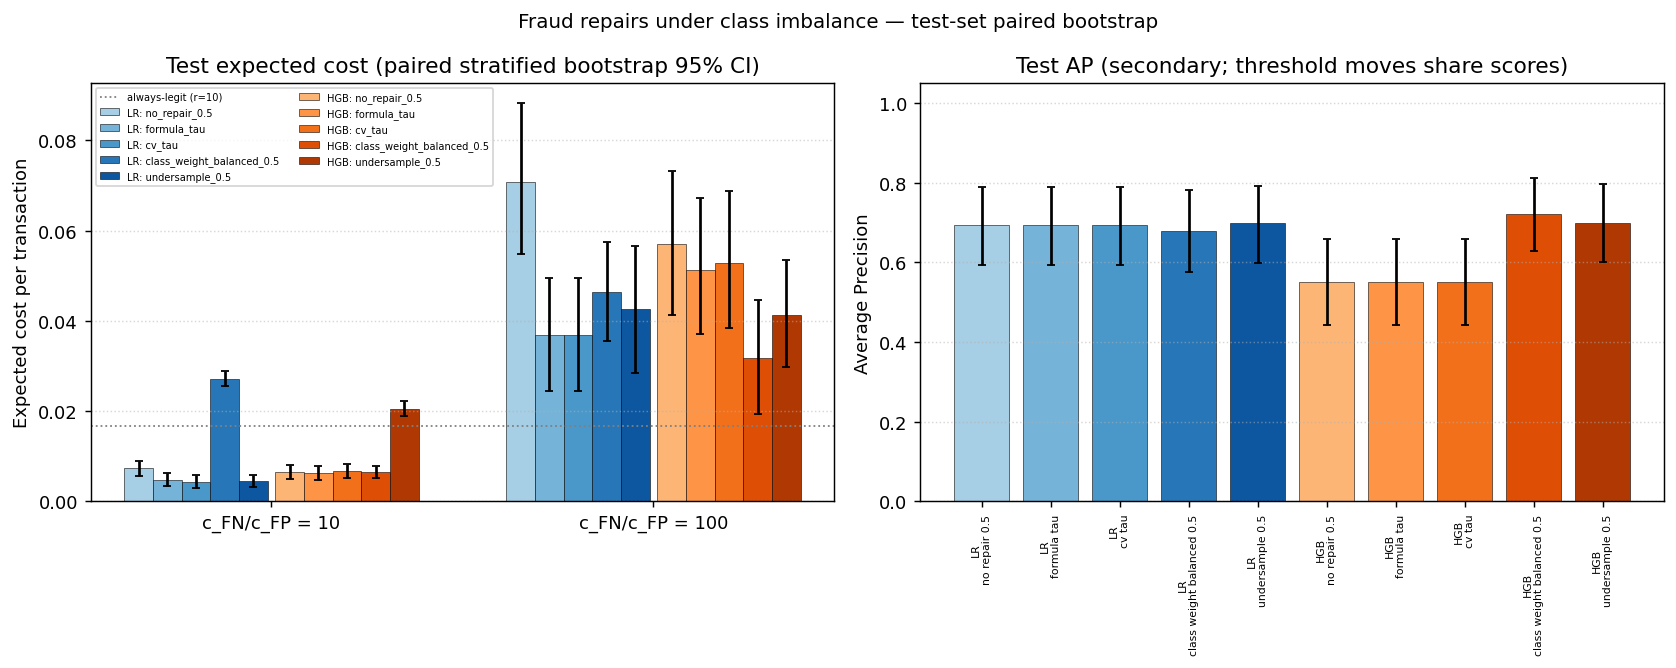
\includegraphics[width=\linewidth]{figures/fig_cost_ap.png}
\caption{Test expected cost (left) and AP (right) with paired stratified bootstrap 95\% CIs. Threshold moves share AP with no repair for each model.}
\label{fig:cost}
\end{figure}

\begin{figure}[t]
\centering
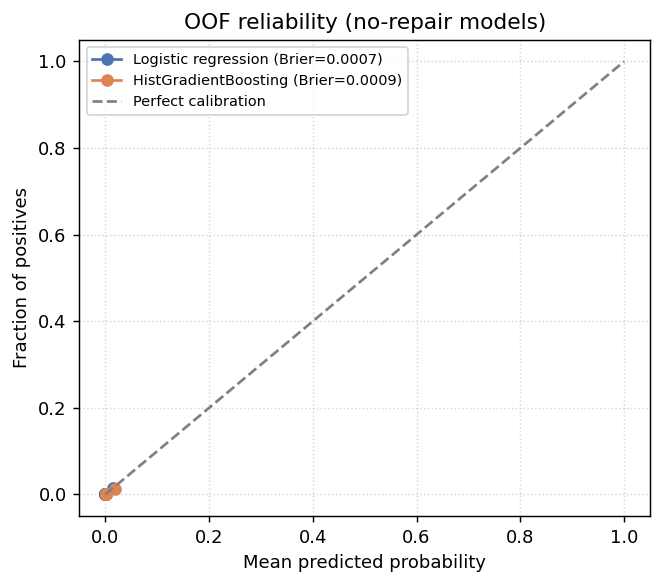
\includegraphics[width=0.95\linewidth]{figures/fig_calibration.png}
\caption{Out-of-fold reliability for no-repair models. Logistic regression is better calibrated (Brier $0.00069$) than HistGB (Brier $0.00093$), consistent with formula $\tau^{\star}$ working well for LR.}
\label{fig:cal}
\end{figure}

Table~\ref{tab:main} and Figure~\ref{fig:cost} summarize the locked test evaluation.
Always-legitimate costs on the test base rate are about $0.0167$ ($r{=}10$) and $0.167$ ($r{=}100$); all serious methods beat these.

\paragraph{Ratio 10.}
Logistic CV-chosen $\tau$ has the lowest mean cost ($0.0043$).
Its interval overlaps formula $\tau^{\star}$ ($0.0047$) and undersampling ($0.0044$): we call these a \textbf{tie} for practical purposes.
Class-weighted logistic regression is clearly worse ($0.027$), driven by very low precision ($\approx 0.055$) despite high recall.
HistGB threshold repairs do not beat the best logistic threshold repairs at this milder asymmetry.

\paragraph{Ratio 100.}
Class-weighted HistGB attains the lowest mean cost ($0.0318$) with the highest AP among all cells ($0.721$).
Logistic formula and CV-chosen thresholds are tied with each other at $0.0369$ (same cut $\tau^{\star}$), and their intervals overlap the HistGB class-weight interval only partially at the upper end---point estimate favors HistGB+weights, but with $95$ test frauds we treat strong claims cautiously.
Undersampled HistGB is worse at ratio~10 (many false positives) and only middling at ratio~100.

\paragraph{AP as a second panel.}
As predicted, formula and CV thresholds inherit the no-repair AP exactly ($0.693$ for LR; $0.551$ for weak no-repair HistGB).
AP alone would have missed the large cost drop from moving LR's threshold and would have understated the value of class-weighted HistGB relative to LR thresholding at ratio~100.

\paragraph{Calibration.}
Figure~\ref{fig:cal} shows that no-repair logistic regression is better calibrated out of fold than HistGB, which helps explain why $\tau^{\star}$ matches the CV-chosen cut for LR at ratio~100, while HistGB's CV-chosen cut drifts lower.

\section{Limitations}
The cost ratios are hypothetical, not bank estimates.
CV-chosen thresholds are selected from in-sample training probabilities (mildly optimistic for the cut itself; test cost remains honest).
With only $95$ test frauds, bootstrap intervals are wide; several comparisons are ties.
We do not stack repairs (e.g., weights plus a new threshold) and we omit oversampling/SMOTE by design.
Hyperparameter selection by AP is itself slightly unstable in flat regions of the grid; we report the argmax but treat nearby settings as near-ties.

\section{Conclusion}
Under severe class imbalance, the best fraud \emph{repair} depends on the cost ratio and the model.
When false negatives are moderately more costly ($r{=}10$), moving the logistic threshold (formula or CV-chosen)---or undersampling logistic regression---minimizes expected cost and beats class weighting.
When misses are much more costly ($r{=}100$), class-weighted histogram gradient boosting achieves the lowest expected cost in our locked test evaluation.
AP is necessary for ranking quality but insufficient as a headline metric for threshold and prior-shift repairs.
Future work includes stacking diagnostics (weights then retuned $\tau$) only if predeclared, and richer calibration fixes before applying $\tau^{\star}$ to tree ensembles.

\begin{thebibliography}{9}
\bibitem{elkan2001foundations}
C.~Elkan.
\newblock The foundations of cost-sensitive learning.
\newblock In \emph{IJCAI}, 2001.

\bibitem{he2009learning}
H.~He and E.~A.~Garcia.
\newblock Learning from imbalanced data.
\newblock \emph{IEEE TKDE}, 2009.
\end{thebibliography}

\section*{Reproducibility}
Code: \url{https://github.com/Urav-Dalal/ESE5420_Final_Project}.
Run \texttt{python experiments\_draft.py} from the repo root (caches OpenML data under \texttt{data/}; writes figures and JSON under \texttt{results/}).
This early draft uses those artifacts.

\end{document}
